\documentclass[11pt,a4paper]{article}
\usepackage[top=3cm, bottom=3cm, left=2.5cm, right=2.2cm]{geometry} %geometry of page
\usepackage[hidelinks]{hyperref} %reference links
\usepackage{fancyhdr} %header and footer control
\usepackage{minted} %source code syntax highlighting
\usepackage{qrcode} %qrcode links
\usepackage{tikz} %diagrams

\linespread{1.3}
\emergencystretch 3em

% Set Header and Footer
\fancyhead{}
\fancyhead[L]{\textbf{Lab 6: Motor control}}
\fancyhead[R]{d.s.brennan@sheffield.ac.uk}
\fancyfoot{}
\fancyfoot[L]{\thepage}
\fancyfoot[R]{MAC 233 Arduino Labs, School of MAC, University of Sheffield}

% Create Document
\begin{document}
\pagestyle{fancy}

\section*{Prerequisites}
This worksheet builds upon the Lab 5 worksheet. You will have needed to complete the Lab 5 worksheet before you can continue with this lab. Out of your Arduino pack, you will need: 1 Arduino, 1 A3144 hall effect sensor, 1 Servo, 1 LED, 1 $10K\Omega$ resistor, 1 $220\Omega$ resistor, and 8 jumper cables.

\section*{Objectives}
There are two objectives of today's lab; expand the control system sketch you built in Lab 5 to control the Electronic Speed Controller (ESC) through pulse length values, and to experiment with different power curves. This lab is different from the previous labs you have completed, as only partial code help is given; however, like the previous labs there is a complete example linked in the help section below.

\section*{Controlling an ESC through pulse lengths}
\label{sec:microseconds}
As discussed in previous labs, an ESC (or servo in our case) attached to an Arduino is controlled through Pulse Width Modulation --- please refer to the electronics PWM lecture. Each PWM capable device has a minimum and maximum length of pulse (in milliseconds) which maps to the devices output range. In the case of a servo, the minimum pulse length equals 0 degrees and the maximum pulse length equals 180 degrees. The Arduino servo library subsequently maps the range from the minimum and maximum pulse length into degrees for simple servo control.\\

\noindent
In our previous labs, we haven't had to set the minimum and maximum pulse length as the Arduino `servo' library has inbuilt defaults: 0.544ms for the minimum and 2.4ms for the maximum. Whilst these default minimum and maximum pulse length values work fine for our servos, they don't work when we are controlling an ESC. The ESC's we are using in the e-bike rigs next semester have three states: neutral, full reverse throttle, and full forward throttle. A typical PWM range for an ESC is 1ms to 2ms. As such, the ESC's that you will use on the e-bike rig have had neutral set to 1.1ms and full forward throttle as 2ms --- \textit{Note: While the above description of pulse length gives the units as milliseconds, the Arduino `servo' library uses microseconds}.\\

\pagebreak
\section{System Functionality}
\label{sec:functionality}
The functionality of this system is the same as described in Lab 5: \textit{ create a basic e-bike control system, so that whenever a magnet passes the field of the hall effect sensor, we increase the output power to the ESC as long as the last hall effect interrupt was within 1.5 seconds. If the aforementioned conditions are not met, power down the ESC to the neutral position.}. The only difference in this Lab, is that instead of giving that output power in degrees, it will now be the value in microseconds of the pulse length.\\

\section{Changing the existing code}
Firstly, open your sketch from the Lab 5 worksheet into Arduino IDE. Once this is open, save the sketch under a new name (`File'\textrightarrow `Save As'). This will make sure you still have a copy of the sketch from Lab 5. The code changes required can be summed up into four sections: 1 - change the ESC variables (global scope), 2 - set the pulse length range (`setup' scope), 3 - update logic range (`setup' \& `loop' scope), 4 - change the written values to the ESC (`setup' \& `loop' scope). While this is all the code required to meet the new specification of the system, the code will only be given for methods you haven't seen before.

\subsection{Change ESC Variables}
The first section we need to change is the ESC variables in the global scope: `$esc\_step\_up$' and `$esc\_step\_down$'. As the ESC control in the previous labs was based in degrees, floats (decimal numbers) were used to provide granular control of the output, as the pulse length is based in microseconds, we can move back to ints (whole numbers) to control the step up and down of the ESC power output.\\
\vspace{-1.75em}
\inputminted{arduino}{./src/1-esc-constants.txt}
\vspace{.75em}

\subsection{Set the pulse length range}
The second implementation change is to provide the minimum and maximum pulse length in microseconds to the Arduino `servo' library. This is done by passing the minimum and maximum values when you attach the `servo' library to the `$ESC\_PIN$' in the `setup' scope: \mintinline{arduino}{esc.attach(ESC_PIN, 1100, 2000);} --- in our case, this is 1100 (1.1ms) and 2000 (2ms). There is only one occurrence within the sketch that needs updating.\\

\noindent
\textit{Hint 1 --- line 65 in the linked help version.}

\subsection{Update logic range}
Throughout the logic of the sketch, the code references the endpoints (the two extremes) of the range. Previously, when the logic was operating in degrees this was $0$ and $180$. Now that we are controlling the ESC in pulse length values, the endpoints are now $1100$ and $2000$. These new values need referencing in the sketch for this Lab. There are five occurrences within the sketch that need updating.\\

\noindent
\textit{Hint 1 --- the logic appears in both the `setup' and `loop' scopes.}\\
\noindent
\textit{Hint 2 --- lines 66, 88, 91, 94, and 97 in the linked help version.}

\subsection{Change the value written to the ESC}
The last update to your sketch, is to change how you write the values to your ESC. Previously, you would use `\mintinline{arduino}{esc.write(0);}' (where 0 is the value in degrees) to change the output value to the ESC. Now that we are working in pulse lengths, we need to instead use `\mintinline{arduino}{esc.writeMicroseconds(0);}' (where 0 is the value in microseconds). There are two occurrences within the sketch that need updating to this new method.\\

\noindent
\textit{Hint 1 --- the logic appears in both the `setup' and `loop' scopes.}\\
\noindent
\textit{Hint 2 --- lines 66 and 100 in the linked help version.}

\section*{Try it out on your Arduino}
You now should be able to compile your sketch (`Sketch'\textrightarrow `Verify/Compile') and then upload to your Arduino (`Sketch'\textrightarrow `Upload'). You should now be able to pass the magnet across a side of the hall effect sensor, and every time you do, it should light up the LED, and your servo should start to power up. When you stop passing the magnet past your hall effect sensor, the servo will start to power down. You will notice that the range of movement on the servo is no longer the full 180 degrees. Once you have a working sketch, move onto the next section below.

\section{Default power curve}
You will be provided the default sketch for operating your gearbox on the e-bike rig for next semester. You are allowed to change certain none-safety associated sections of the code to enhance the performance of your gearbox. One of these such sections, is the ESC output power curve. During the test day, the rig will measure how many rotations of the virtual wheel you achieve within a 30-second window --- the window starting when the criteria for power being sent to the ESC is reached.\\

\noindent
\textit{\textbf{Note:} Modifying sections of the code that are labelled as safety logic --- they have a `DO NOT CHANGE' comment --- will result in an instant disqualification on test day}.\\

\noindent
As the default code has been written to work on any gearbox, the power curve from the code is glacially slow to operate a modicum of `mechanical sympathy' on your gearbox. The control system has no knowledge of how you have designed your gearbox; therefore, the system must be gentle and slow to minimise the torque and stress placed on your gearbox. If you have designed your gearbox to take the maximum torque from 0 seconds without drawing more current than allowed, then you can change your control system to suit.\\

\begin{figure}[ht]
    \begin{center}
        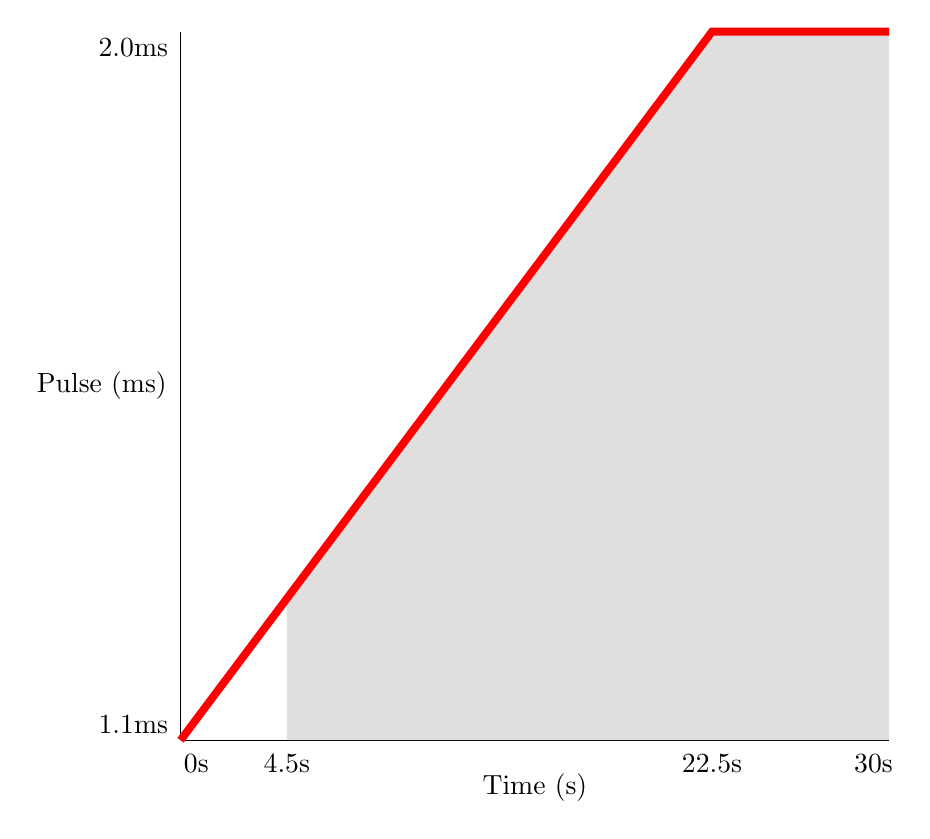
\begin{tikzpicture}[
            axis/.style={draw=black},
            power/.style={draw=red, line width=1mm},
            area/.style={fill=gray, fill opacity=0.25}
        ]
            % axis
            \draw[axis] (0, 0) -- (0, 9);
            \draw[axis] (0, 0) -- (9, 0);
            % numbers
            \node at (-0.6, 0.2) {1.1ms};
            \node at (-1.0, 4.5) {Pulse (ms)};
            \node at (-0.6, 8.8) {2.0ms};
            \node at (0.2, -0.3) {0s};
            \node at (1.35, -0.3) {4.5s};
            \node at (6.75, -0.3) {22.5s};
            \node at (4.5, -0.6) {Time (s)};
            \node at (8.8, -0.3) {30s};
            % area
            \path[area] (1.35, 0) -- (1.35, 1.8) -- (6.75, 9) -- (9, 9) -- (9, 0) -- (1.35, 0);
            % lines
            \draw[power] (0, 0) -- (6.75, 9) -- (9, 9);
        \end{tikzpicture}
    \end{center}
    \caption{Pulse length output from default code over time.}
    \label{fig:output-time}
\end{figure}

\noindent
Figure \ref{fig:output-time} depicts the default power curve of the standard e-bike control system code. The red line indicates the power output value sent to the ESC, and the grey area below the red line indicates when the gearbox will be turning. Given that the `loop' function will pause for 50 milliseconds every iteration --- one of the safety values that cannot be changed --- we can calculate how long it will take to reach full forward power. With a `step up' in the pulse length of 2 microseconds every 0.05 seconds and a range of 900 microseconds (1100 microseconds for neutral, 2000 microseconds at full forward power), it will take 22.5 seconds of the 30-second window to reach full forward power. This means with the default code, you will only have 7.5s of full forward power.\\

\noindent
You may also notice, that according to Figure 1, the gearbox won't be turning for the first 4.5 seconds of the 30-second window. This is because the rig you will be using has a sensorless ESC and motor. In a sensorless setup, the ESC needs a roughly 20-30\% boost from the base pulse length to start turning the motor. The exact value will depend upon your clearances in your gearbox and how much force is required to make it initially move.

\subsection{Change the power curve}
Given the information in the previous section, there are two main areas within the code that will allow you to have full forward power for a larger percentage of your 30-second window.

\begin{enumerate}
    \item Modifying the code to reduce the 4.5-second delay to 0 seconds.
    \item Changing the power curve to get to full forward power sooner in your 30-second window.
\end{enumerate}

\noindent
Your task now is as a group, try to implement different methods for fixing the above highlighted problems in your Lab 6 sketch. The default e-bike control system code you will be given next week operates under the exact same principles as the code you have built in this lab; therefore, you will be able to migrate your methods from today's lab into the final control system code which forms part of your assessment on the test day. As a result, there are no answers given in today worksheet on how to do this. You can as always, ask questions from any of the helpers in the Lab.\\

\noindent
\textit{\textbf{Note:} Setting the code to output full forward power from 0 seconds will most likely result in gears being stripped or pulling more amps than the allowed limit}.\\

\pagebreak
\section*{Help}
If you are having issue compiling the project or don't understand where each section goes, you can see a complete version of the sketch with additional source code comments at \url{https://github.com/dsbrennan/mac-233-arduino-labs/blob/main/lab-6-motor-control/lab-6-motor-control.ino}.

\begin{center}
    \qrcode[hyperlink, height=3cm]{https://github.com/dsbrennan/mac-233-arduino-labs/blob/main/lab-6-motor-control/lab-6-motor-control.ino}
\end{center}

\end{document}